Una branca dell'informatica che sta acquisendo sempre più rilevanza è quella che riguarda l'analisi dei programmi: \\conoscere certe proprietà e comportamenti di un programma prima che venga eseguito (\textbf{analisi statica}) o durante la sua esecuzione (analisi dinamica) può mettere in condizione di poter fornire garanzie circa il suo consumo di risorse, la sua correttezza, la sua sicurezza o la sua l'efficienza.
Queste garanzie, in alcuni ambiti critici, possono risultare imprescindibili ma riuscire a dimostrare queste proprietà non è un'attività banale a causa delle limitazioni teoriche su cui di basa l'informatica stessa.

Uno dei più grandi limiti posti dalle fondamentali intuizioni di Alan Turing riguardo l'analisi dei programmi si evidenzia nell'\textit{halting problem} \cite{Turing1936}: il quesito ``è sempre possibile, descritto un programma e un determinato input, stabilire se il programma in questione termina o continua la sua esecuzione all'infinito?'' è \textit{non decidibile}.
Si dice \textit{indecidibile} un problema per il quale non esiste alcun programma che possa determinare, per ogni possibile input, se la risposta sia positiva o negativa in un tempo finito.

Questo risultato porta ad esempio ad intuire come sia inoltre impossibile calcolare l'intera \textit{semantica concreta} di un programma, infatti, essa rappresenta l'insieme (infinito) di tutti i possibili flussi di esecuzione in tutti i possibili ambienti di esecuzione (Figura~\ref{fig:semantica_concreta}).

\begin{figure}[ht]
    \centering
    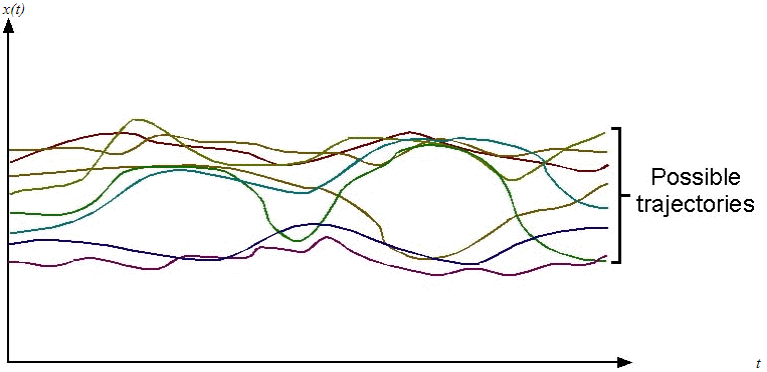
\includegraphics[width=0.47\textwidth]{figures/semantica_concreta.png}
    \caption{Rappresentazione delle possibili esecuzioni di un programma tramite curve che mostrano l'andamento dei valori in input, dello stato e dell'output in funzione del tempo.}
    \label{fig:semantica_concreta}
\end{figure}

Posti questi limiti, esistono comunque alcuni modi per affrontare il problema della verifica della proprietà di \textit{safety} che risulta essere tra quelle di maggiore interesse.
Per cercare di raggiungere tale obiettivo l'analisi dinamica considera direttamente la semantica concreta cercando di stabilire se una qualsiasi delle sue traiettorie intersechi una zona rappresentante uno stato di errore (Figura~\ref{fig:forbidden_zone}).
\begin{figure}[ht]
    \centering
    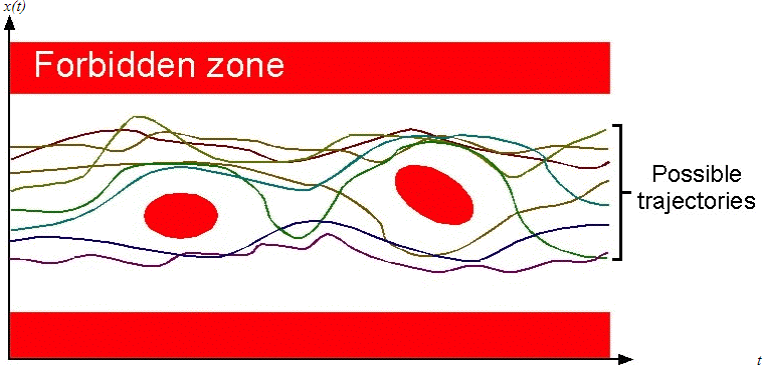
\includegraphics[width=0.47\textwidth]{figures/forbidden_zone.png}
    \caption{La \textit{forbidden zone} rappresenta gli stati in cui l'esecuzione del programma è in errore.}
    \label{fig:forbidden_zone}
\end{figure}

Tuttavia, la maggior parte delle tecniche che si concentrano sull'analisi a \textit{runtime} soffrono del problema dell'\textit{Absence of Coverage}: a causa dalla natura infinita della semantica concreta, non è possibile assicurare la proprietà di \textit{safety} perché, con questo approccio, verranno sicuramente tralasciati dei possibili flussi di esecuzione che potenzialmente potrebbero portare ad uno stato di errore.

In certi ambiti non critici questo approccio può risultare sufficiente ma, dove tale proprietà è di cruciale importanza, non è possibile lasciare spazio ad incertezze.
Perciò, la branca della verifica del software che sembra più adatta agli ambiti critici risulta essere l'analisi statica, approccio speculare rispetto a quello appena visto, che riesce ad abbassare il livello di incertezza sotto le più stringenti specifiche tramite ``\textit{approssimazione}''.

\newpage

\subsubsection{Interpretazione Astratta}
L'\textbf{Interpretazione Astratta} \cite{AbsIntNutshell} è un metodo formale dell'\\analisi statica che consiste nel considerare un sovrainsieme di tutti i possibili flussi di esecuzione di un programma (detto \textit{semantica astratta}) in modo che, se una proprietà risulta verificata per esso, lo sarà sicuramente anche per l'interezza della semantica concreta Figura~\ref{fig:semantica_astratta}.

\begin{figure}[ht]
    \centering
    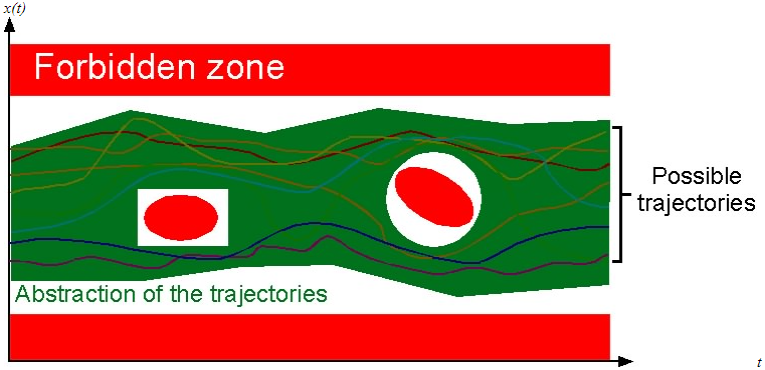
\includegraphics[width=0.47\textwidth]{figures/semantica_astratta.png}
    \caption{L'area verde rappresenta la \textit{semantica astratta}: un'approssimazione per eccesso della \textit{semantica concreta}.}
    \label{fig:semantica_astratta}
\end{figure}

I due rischi principali della definizione della semantica astratta risiedono nel processo di approssimazione.
Infatti, è possibile infrangere la proprietà di \textit{soundness} effettuando \\un'approssimazione eccessivamente restrittiva o, all'opposto, avere falsi positivi durante l'analisi a causa di un'\\approssimazione troppo ampia che interseca la zona di errore nonostante il programma non possa in alcun modo raggiungere quello stato (falso positivo).

Nonostante le limitazioni, questo approccio risulta essere effettivamente utilizzato, ad esempio  attraverso l'analizzatore statico Astrée \cite{AbsIntProfile}, da aziende come Airbus, Bosch, ESA ed altri per rispettare gli standard di sicurezza come il sopracitato DO-178C \cite{AbsIntSuccess}.